\chapter{Background}

This chapter will outline the information needed for better understanding of the idea of the project and its underlying processes.

\section{Spiking Neural Networks}

An \emph{artificial neural network}(ANN) is defined as a computational model inspired by the structure and functional aspects of biological neural networks.\cite{ActFunc}
It is an adaptive system that consists of \textbf{neurons}, its basic computational units, that are connected with each other via \textbf{synapses}.
Modern neural networks are mostly used as non-linear statistical data modeling tools to find patterns between inputs and outputs.\cite{Bar-Yam2003}

\emph{Spiking neural network}(SNN) - is a third generation neural network that comprises within itself not only concepts of neuronal and synaptic states, but 
also time.\cite{Maass1997} As a result of putting emphasis on time as an acting property, a much higher level of realism is achieved in simulations,
making SNNs particularly useful for research in such areas as brain activity or neural computation.

\subsection{Artificial and Spiking Neurons}

In order to distinguish between different generations of neural networks, one would need to take into account type of neurons, as they define the type of network.

\begin{figure}[h]
\begin{center}
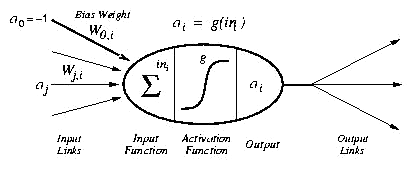
\includegraphics[scale = 0.6]{images/neuron_model.png}
\end{center}
\caption{A graphical model of a simple artificial neuron\cite{Philosophy}}
\end{figure}

Typical neural networks consist of a number of computational units, \emph{artificial neurons}. An \emph{artificial neuron} is a model of a mathematical 
function or an abstraction of biological neurons\cite{Harmon1959}, that given several inputs, derives a value based on the sum of this collection of inputs 
and built-in function, and returns this value as an output, essentially acting as an axon of a real neuron. Artificial neurons differ depending on their 
specific model, such as McCulloch-Pitts or linear-threshold function. These models define a set of properties that a particular neuron possesses, such as 
transfer (or activation) function.

\begin{figure}[h]
\begin{center}
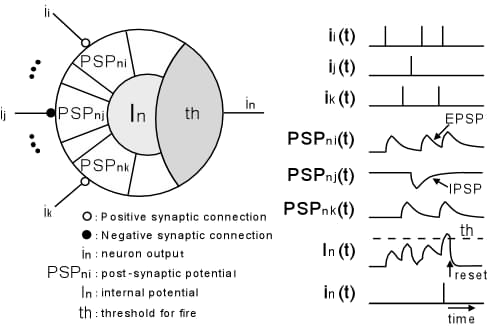
\includegraphics[scale = 0.8]{images/spiking-model.png}
\end{center}
\caption{A graphical model of a spiking neuron\cite{HidekiTanaka2009}}
\end{figure}

However, spiking neural networks are quite different in nature and, specifically, in structure of their computational units from artificial neural networks. SNNs consist of \textbf{spiking neurons} 
that aim to model the activity of real biological neurons, that is to make an abstraction which is as close as possible to the original. A \emph{spiking neuron} instead of
having set time period of emission, fires a \textbf{spike} - a very short signal that remains at its peak value for about a millisecond. Firing in spiking neurons is caused
by changes in membrane potential as well as resulting from time-based activation function. The signal is transferred to other neurons, in turn, increasing or decreasing their
membrane potential. However, since signals do not vary in value, the information is transferred via a collection of spikes, called a \emph{spike train}. Through the spike train
it is relatively easy to obtain the timing and number of spikes, therefore, these two variables hold the actual data.\cite{WulframGerstner2002} By possessing these qualities, networks 
built from spiking neurons obtain a significantly larger computational power than that of same-sized artificial neural network.\cite{Maass2003}

\subsubsection{Activation Function}

An activation function is usually an abstraction that represents the firing rate of the cell, that is dependent on the sum of inputs as well as on time.\cite{ActFunc} In spiking neural networks,
this function does not output a binary set of values, but is rather calculated through a set of differential equations that depend on the input current and, if implemented, time.

\subsubsection{Spiking Neuron Models}

In order to make computer simulations more analytically and computationally tractable, there have been derived several types of neuron models that could be used as best approximation of the actual
biological neuron behaviour. Here are some of them.

\begin{itemize}

\item \textbf{Integrate and Fire}

\emph{Integrate and Fire}(IF) model is a simple and relatively accurate representation of the actual biological neuron.
It divides the behaviour of membrane potential into two parts: long periods of \emph{integration} and short firing of \emph{spikes}. The activation function for this kind of neurons is
a time derivative of the law of capacitance, with a refactoring time added to limit the speed of firing:
\begin{center}
\begin{equation}f(I) = \frac{I}{C_{m}V_{th} + t_{ref}I}\end{equation}
\end{center}
where $C_{m}$ stands for membrane capacitance, $V_{th}$ is threshold voltage and $t_{ref}$ is refactoring time. Therefore, the rate of firing is directly proportional to the input current.\cite{WulframGerstner2002}

However, if not modified, this model does not implement time-dependent memory. Moreover, it also lacks details in representation of biological neurons, as most of the biophysiological 
processes are simplified. For example lagging of sodium channel activation present in Hodgkin-Huxley model is absent in IF.

In order to compensate for the lack of the time-dependent memory, there has been derived an enhanced version of IF model - \emph{Leaky Integrate and Fire} (sometimes refered to as \emph{AdEx} - short for Adaptive Exponential integrate and fire model).\cite{IFModel} This particular implementation relies on two differential equations - one describing the dynamics of membrane coupled with an exponential voltage dependance:

\begin{center}
\begin{equation}C\frac{dV}{dt} = -g_{L}(V-E_{L}) + g_{L}\Delta_{T}exp(\frac{V-V_{T}}{\Delta_{T}})-\omega + I\end{equation}
\end{center}

And another one used for deriving adaptation:

\begin{center}
\begin{equation}\tau_{\omega} \frac{d\omega}{dt} = a(V-E_{L}) -\omega \end{equation}
\end{center}

where V is the membrane potential, $\omega$ - the adaptation variable, I - the input current, C - the membrane capacitance, $g_{L}$ - the leak conductance, $E_{L}$ - the leak reversal potential, $V_{T}$ - the threshold, $\Delta_{T}$ the slope factor, a the adaptation coupling parameter and $\tau_{\omega}$ is the adaptation time constant.

\item \textbf{Hodgkin and Huxley}

\emph{Hodgkin and Huxley}(HH) model aims to incorporate an exhaustive description of a real biological neuron - therefore, requiring a large number of parameters to operate.
As opposed to IF, HH model uses nonlinear differential equations in its activation function to determine the membrane charasteristics and, therefore, provide the closest 
biophysical representation of a biological neuron.\cite{Hodgkin1952} The interpretation of this model operates using several equations for \emph{voltage-gated ion channels}:

\begin{center}
\begin{equation}g_{n}(V_{m}) = \bar{g}_{n} \varphi^{\alpha} \chi^{\beta}\end{equation}
\begin{equation}\dot{\varphi}(V_{m}) = \frac{1}{\tau_{\varphi}}(\varphi_{\infty} - \varphi)\end{equation}
\begin{equation}\dot{\chi}(V_{m}) = \frac{1}{\tau_{\chi}}(\chi_{\infty} - \chi)\end{equation}
\end{center}

Here $\varphi$ and $\chi$ represent the activation and inactivation functions.
ELABORATE

\item \textbf{Izhikevich model}

\emph{Izhikevich neuron model} is aiming to produce a plausible representation, close to HH, of a biological neuron, while maintaining the computational power and efficiency of an IF model.
It has several improvements over IF model, such as enhancing the activation function for the purpose of more accurate spike firing representation, which is done by introducing more 
types of spiking periods and give the implementation.\cite{Izhikevich2003}
ELABORATE

\end{itemize}

\subsection{Synapses}

\emph{Synapses} in spiking neural networks represent dendrites in biological neural systems, making directed connections between spiking neurons. 
Therefore, synapses act as the main transmitters of spikes within the network, contributing to the connectionist approach, the main paradigm of neural networks.

\subsubsection{Synaptic Plasticity}

\emph{Synaptic plasticity} is the ability of a given synapse to change the number of receptors depending on the use.\cite{WulframGerstner2002} This represents quite an
important part of the neural network model, as it is a part of real-time alterations that occur during the actual simulation.

Spiking neural networks rely on \emph{spike timing dependent plasticity}(STDP) model for simulating plasticity, as most of information transmitted in SNNs is dependent not on 
the power of signals but rather on their timing and number. STDP rules divide the spikes occuring onto pre- and post-synaptic, determining the changes in the action potential that
they bring in. Consequently, these parameters control the extent of synaptic modification.\cite{SenSong2000}

\subsection{Topology}

Topology of a neural network is essentially its layout, that displays the connections between the neurons. Topology plays critical role, when 
the neural network is mapped onto the computational clusters, as it helps distinguish an optimal way of allocating neurons between the nodes,
and by doing this significantly increase the efficiency of communication.

\begin{figure}[h]
\begin{center}
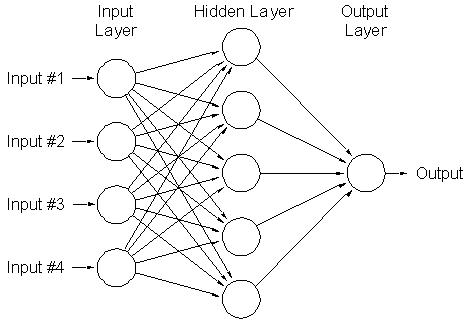
\includegraphics[scale = 0.3]{images/topology.png}
\end{center}
\caption{Topology of a feed-forward neural network\cite{Tan2006}}
\end{figure}

\section{Spiking Neural Network Simulators}

In order to give a better outlook on the field of spiking neural network simulation, this section will cover some of the state of the art solutions present to date.

\subsection{NeMo}

\emph{NeMo} is a spiking neural network simulator aimed at real-time simulation of large-scale neuron systems with the use of highly parallel GPUs.\cite{AndreasK.Fidjeland2009}
NeMo's main purpose is to produce simulations that would be particularly useful for research, therefore, main emphasis in this tool is put onto scalability and real-time aspects
of produced simulations.

NeMo is the main platform of MPI implementation for this project. The main goal is to improve inter-neural communication between computational clusters within NeMo.
At the same time, neuron mapping should be changed to ensure efficient communication during the simulation. NeMo simulator is going to be shown in more details in the following section.

\subsection{Brian}

Another solution, \emph{Brian} aims for bigger flexibility and ease of use, therefore making it more suitable for teaching purposes. \cite{Goodman2008} This
particular simulator will provide a good example of an spiking neural network simulator, and as it is easy to operate, will be useful for learning main concepts
of SNN in detail.

\subsection{SpikeNET}

\emph{SpikeNET} is a spiking neural network simulator created for large-scale integrate-and-fire networks simulations.\cite{ArnaudDelorme1999} As the main aim of this project is to
achieve the highest possible number of neurons hosted and computed simultaneously, this solution requires a very high level of parallelism in order to operate.
Therefore, findings from this project would be useful later in the project, when the focus is going to be on the scale of computations.

\subsection{Blue Brain Project}

Initiated in cooperation between IBM and EPFL, the \emph{Blue Brain Project} aims to produce a virtual brain in a supercomputer, Blue Gene, provided by IBM.\cite{BlueBrain} Computational power
required for the operations is immense, however, supercomputing technology gave neuroscientists a set of tools to solve this problem. The Blue Brain simulator is
a very interesting project, and due to exceptionally difficult task of reducing workload across the stations - it will be particularly useful at the stage of MPI development.

\section{NeMo Architecture}

The main project platform, NeMo, has most of its functionality concentrated around three classes - \emph{Configuration}, \emph{Network} and \emph{Simulation}.
ELABORATE


\section{Distributed Computing}

As the main objective of the project is to enhance communication efficiency between neurons in the spiking neural network, use of distributed computing plays crucial
role in its achieving. In this context, distributed computing means parallelization of tasks across the connected system and providing efficient communication medium
between separate computational clusters.

\subsection{Parallel Computing}

\emph{Parallel computing} is a form of computation where most of calculations are carried out simultaneously.\cite{G.S.Almasi1989} In order to achieve this, large problems
are divided into smaller independent parts that are carried out by separate computational units, with feeding the results either into the main cluster or holding it for further
computations. The rise of this particular field is due to the need in high-performance computing, especially in the light of frequency scaling becoming more and more
limited because of power consumption.\cite{Kumar2002}

Due to the nature of this project, a high degree of parallelism is crucial, in order to maintain the highest possible speed of simulation - the matter is that simulation would
be split between several clusters (\emph{nodes}) which, depending on the mapping, will operate independently, after receiving the information from main node at the start.
PICTURE

\subsection{Message Passing Interface}

\emph{Message Passing Interface} (MPI) is a language-independent protocol which acts as a communications medium for a group of processes.\cite{mpi} MPI's main function is to provide
a solid communication channel between the processes in a highly parallelised system, thus, enhancing efficiency of this system. Message passing programs are written in Fortran and 
C, with the use of built-in functions.

Currently NeMo has an MPI implementation within it, however, it is not the most optimal one. The main idea behind parallelisation in this project is that neurons are allocated, 
using mapping algorithm, between several computational nodes, which are communicating with each other with the use of MPI. Therefore, one of the main objectives will be to 
create an MPI layer inside system, that would increase the speed of computations by enhancing quality of inter-cluster communication.

There are currently several implementations of MPI to date, so here is a brief overview of available solutions.

\subsubsection{Open MPI}

The \emph{Open MPI Project} is an open-source implementation of MPI-2 maintained by a group of academic, research and industry partners, Open MPI Team.\cite{RichardL.Graham2005} This particular 
implementation aims at compatibility and high performance on all platforms, thus, making it quite easy to install and configure. Open MPI is a useful tool that will help understand 
the underlying concepts of message passing and generally give a good background within this subject area.

\subsubsection{MPICH2}

\emph{MPICH2} is an MPI implementation from Argonne National Laboratory, that aims at high performance and extendability.\cite{W.Gropp1999} The main idea of the project is to make the simulations as
fast as possible, via enhancing the efficiency of communication, therefore, MPICH2 fits well with the aims set, by providing focus on the speed and effectiveness. Another reason to choose 
MPICH2 for this project is that this package is already installed on the lab machines, therefore, saving time for the initial setup.\cite{W.Gropp1999a}

\subsection{Cluster-based approach and Mapping}

One of the most important part of the simulation is the initial \textbf{mapping} of neurons across the hosts, as it will affect the amount of inter-cluster communication and therefore overall efficiency of the system. \emph{Mapping} defines the layout of the resulting system and is directly affected by topology - neurons are split into several groups depending on the number of synapses connecting those. The main idea is to keep the amount of inter-cluster communication to minimum, as it is more expensive in terms of memory and time than communication within the node.

Mapping is defined by topology and hierarchy of the system - most of implementations have a master node, accountable for adding neurons and synapses to particular clusters, however, it is
possible to have a distributed system, were all nodes are equal in resposibility and actions are taken independently.

\subsubsection{Clustering algorithms and research}

Division of large scale networks, if applied correctly, greatly increases performance - making these nets computationally feasible to simulate. Consequently, there have already been several successful attempts of classifying best clustering algorithms. This section will give an insight into the algorithm introduced by Mark Newman which focuses on a specific parameter of the network - \emph{modularity}.

\textbf{Modularity} is a measure of the structure of the network that describes its strength of division into subgroups (\emph{modules})

\subsubsection{Current implementations of cluster-based approach within neural networks}
At the moment there are already a few implementations present that focus on the clusterisation of the neural networks in order to achieve better inter-neuron communication and bigger throughput. 
These are the most notable ones that have a direct connection to my project.

\begin{itemize}
\item{\textbf{Izhikevich's large scale model for simulating mammalian thalamocortical systems}}

The work by Eugene Izhikevich\cite{EugeneM.Izhikevich2008}, though being mostly focused on the research of brain dynamics, showed that clusterisation of the network system across several processors would result in much higher throughput rate for a large scale network - million of neurons, tens of millions of neuron compartmentss and almost half a billion synapses. In this particular case C with MPI implementation was used to allow for inter-cluster communication, and it allowed the researchers to scale the time needed for calculation of one sub-millisecond time-step for this type of network to one minute.

\item{\textbf{IBM cortical simulator project (C2)}}

Research conducted by a group of scientists from the IBM Research Centre in Almaden\cite{DharmendraS.Modha2007} focused on creation of a platform capable of simulating cerebral cortex activity. Consequently, due to extremely large scale of simulation - in this project more than 55 million Izhikevich neurons were simulated within one network - and availability of clusters within the centre, a distributed approach was applied with the use of MPI. When applied to this problem, cluster mapping managed to achieve balanced workload across the network, as well as the uniform inhibitory neuron distribution. The reason the latter point mattered in the simulation is the fact that more than 60\% of firing was inhibitory - therefore, incorrectly distributed neuron set would have a significant effect on results.

\item{\textbf{Neuromorphic model for GPGPU cluster}}

Simulator produced by Bing Han and Tarek Taha aimed at the speedup of simulations with Izhikevich and Hodgkin-Huxley neuron models\cite{TarekM.Taha2010}. Use of GPGPUs and multi-threaded MPI provided heterogeneous  clusters and per-cluster computational capacity, and clustering algorithm ensured correct distribution of neurons in accordance to the 2 layers present in the system. As a result, a significant speedup was achieved in computation, factor of 177.0 for Hodgkin-Huxley and 24.6 for Izhikevich neurons, for the task of image recognition.
\end{itemize}
